%加入更多图片
%加入页眉
\documentclass{article}
\usepackage{hyperref}
\usepackage{multirow}
\usepackage{array}
\usepackage{xeCJK}
\usepackage{listings}
\lstset{
	basicstyle = \small\ttfamily,
	breaklines = true,
	frame = single,
	language = python,
	tabsize = 2,
	showspaces = false,
	showstringspaces = false,
	breakindent =1.1em,
}
\setCJKmainfont{SimSun}

\title{Y86流水线模拟器的实现\\计算机原理项目报告}
\author{游沛杰 13307130325}
\begin{document}
\maketitle
\tableofcontents
\newpage

\section{背景介绍}
\indent\indent
在本次项目实验中,我们需要实现一个Y86模拟器,能够正确的流水线化模拟执行课本(CS:APP\cite{1})第4章介绍的Y86指令,并将执行过程和程序运行结果通过图形界面的方式可视化。同时可以帮组我们更好理解课本介绍的知识。我认为这次项目的目的是忠实还原CPU处理Y86汇编程序时候的状态,所以有时候考虑问题会从硬件方面出发。

\section{工作原理}
这里分指令集,流水线阶段,流水线异常处理等部分来介绍
\subsection{指令集}
实现了书本上介绍的全部Y86指令,如下

\begin{center}
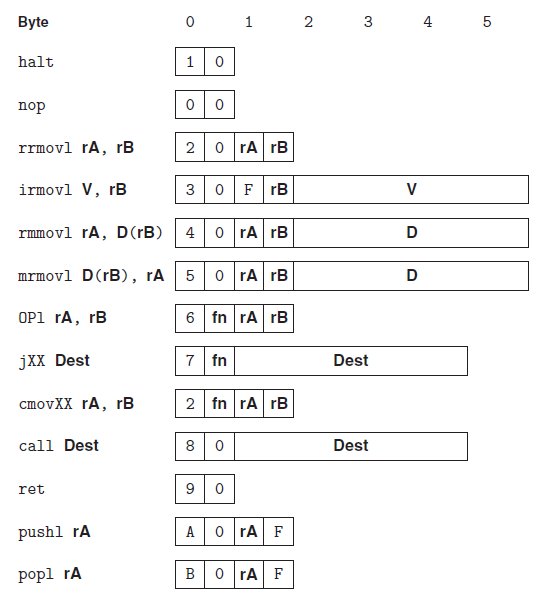
\includegraphics[width = 10cm]{1.png}
\end{center}

其中,地址的形式为D(rB),而指令跳转使用绝对地址的方式(比如jmp 0x123,那么下一条要执行的指令就是0x123开始的指令,而不是pc+0x123或者pc+0x123+0x2)。

数据存储使用小端法。\cite{3}

另外需要说明几点:
\begin{enumerate}
\item 书本上的halt和nop对应的机器码不明确(见第二版英文书P338和P384,前后矛盾)。所以在这里,我把10看成是halt指令对应机器码,00看成是nop指令。
\item 样例给出的RNONE=0x8,而书本上是0xF,在这里我们使用的是0xF
\item 当fetch到的指令发现不需要常数valC的时候,程序不会读取后面的内容,并把valC设成0,而样例结果会\underline{把后面的指令当成常数读入},并没有什么用。
\end{enumerate}
\subsection{PIPELINE}
我实现的流水线分成五个阶段(Fetch, Decode, Execute, Memory, Write back)
\begin{enumerate}
\item Fetch      从指令内存中取出指令以及相关信息(rA、rB编号, valC)
\item Decode     读取相关的寄存器的值(rA, rB, RESP的值)
\item Execute    进行算术/逻辑运算
\item Memory     读写内存
\item Write back 将需要更新的寄存器值放回register file中
\end{enumerate}

使用forward+stall/bubble来处理异常情况。
\begin{itemize}
\item forward 将前面阶段中已经计算好的值直接传输到decode阶段
\item stall 不执行更新,但是保留原来流水线寄存器中的值(延迟到以后再更新)
\item bubble 把pipeline register中保存的值重置置为默认值(舍弃当前已在进行的指令操作)
\end{itemize}
\subsection{Memory}
同步RAM,后面有介绍
\section{我的项目概况}
\begin{center}
\begin{table}[!ht]     % 强制在原位显示表格
\centering
\caption{开发环境}
\begin{tabular}{|l|c|c|c|}
\hline
\multirow{2}{*}{主要使用语言} & 内核 & Python 2.7.9\\
\cline{2-3}
 & GUI & PyQt 4.11.3\\
\hline
\multirow{2}{*}{开发平台} & IDE & PyCharm\\
\cline{2-3}
& 操作系统 & Windows 8.1\\
\hline
辅助工具 & GUI界面绘制 & Qt Creator\\
\hline
\end{tabular}
\end{table}
\end{center}

全部代码均作者本人\underline{独立完成},并没有任何抄袭和复制粘贴的成分。

项目的设计和准备阶段从5月16日开始,经历两个星期(其中有另外2个项目需要完成)。从6月1日左右开始投入实际开发。其中核心部分历时4天编写并完成调试,UI部分做了4-5天。

在这个项目之前几天我们还完成了数据库的课程项目(HTML+PHP实现),所以作者这次不想再写web端的UI,试图使用不会的Qt来实现一个桌面端应用程序。虽然界面不一定好看,但是也是一种挑战。

%目录介绍here

\section{内核具体实现}
\subsection{中间变量的实现}
这里的中间变量指的的stage output,通常以小写字母fdemw开头(比如e\_valE)。

对于这些结果,在硬件上相当于一个组合电路,那么我们就用一个函数来实现,其中函数的输入就相当于硬件层面上的接线,组合电路就在函数内部实现其功能,比如下面例子:

\begin{lstlisting}[frame=single]
def f_stat(f_icode, imem_error):
    #   DONE
    #   有优先级?
    if imem_error: return SADR
    if not instr_valid(f_icode): return SINS
    if f_icode == IHALT: return SHLT
    return SAOK

\end{lstlisting}

其中部分stage output只用到了一次
%example
,我们在需要的时候再计算这个结果,以保证程序整体运行速度,而对于在不止一个地方用到的值,我们采用中间变量来保存这些值。
%example
\\
\\
\\
\indent 我们可以发现,Python的语法与课本上的HCL有很多相似之处,比如有in的用法,Python的list理解起来也比较简单,如下语句:
\begin{lstlisting}[frame=single]
def d_srcB(D_icode, D_rB):
    #   DONE
    if D_icode in [IOPL, IRMMOVL, IMRMOVL]: return D_rB
    if D_icode in [IPUSHL, IPOPL, ICALL, IRET]: return RESP;
    return RNONE;
\end{lstlisting}

我们发现Python在这里看起来就和真的硬件描述语言一样,同时十分接近自然语言,给人带来愉悦感!这也是其他语言(比如C++)所没有的
%词穷
。

使用Python是一个正确的选择。
%_(:зゝ∠)_

\subsection{内存的实现}
下面介绍我的“内存”的实现方式。

在Python中,我用一个list对象来保存内存,假设的大小为4k字节(0x1000个地址),对于绝大部分的Y86汇编程序(包括样例程序)足够了。

其中指令以及常数存储从低地址开始存储,程序运行时从高地址开始堆栈,如图。

同时我们假定这是一个同步的内存,也就是在时钟上升沿的时候我们才进行写入操作。
%图here
\\
\\
\\
\indent 在具体的读取内存操作时候,有两种情况
\begin{enumerate}
\item 读指令,这时候程序会判断当前读的是否合法的指令地址
\begin{lstlisting}[frame=single]
def inst_valid(addr):
	return addr in range(0, max_instr_addr + 1)
\end{lstlisting}
思考一下发现并没有在指令区间中,而读出来其实不是指令的例子(只能是Y86汇编代码写错了)。
所以指令译码错误我们放在模拟器主程序中判断,如果指令非法返回一个错误提示。

\item 读数据。在程序开始运行之前,我们甚至都无法判断一个地址放的是指令还是数据,参见样例汇编程序中从地址0x14开始有一个数组:
\begin{lstlisting}[frame=single]
  0x014: 0d000000     | array:	.long 0xd
  0x018: c0000000     | 	.long 0xc0
  0x01c: 000b0000     | 	.long 0xb00
  0x020: 00a00000     | 	.long 0xa000
\end{lstlisting}

说明数据和指令是混在一起的,所以在读取数据时,我们能只判断地址是否越界,不能很好判断这个地址是否落在“数据”的地址范围。
\end{enumerate}


在写入内存的时候,考虑到这是一个同步的RAM,所以不能异步的写入。
我实现的办法是先把这个写操作记录到一个类似于缓冲区的东西里,当在时钟上升沿的时候再修改。

有点类似于Git的stage和commit操作,如果需要修改,我先加入到stage里面,等时钟上升沿再一起commit。如下例子:
%example here

需要注意的是,这种实现方式从原理上与以下程序有所不同
\begin{lstlisting}[frame=single]
next = [0] * 233
while True:
	this = next
	do_something()
	#	从this里面读数据,写到next里面
\end{lstlisting}

这里是有两个内存,\underline{并不很符合硬件的实际},同时如果内存较大,则需要两倍的空间。

而我每次只记录需要写入的地址和数据信息,每个时钟周期都会清空。\\\\
\indent 同时也和下面程序不同
\begin{lstlisting}[frame=single]
this = [0] * 233
while True:
	do_something()
	#	排列读写this的顺序,保证写入以后不会在同一个时钟周期读到。
\end{lstlisting}

上面的简直就是组合逻辑电路,并没有反应真实情况。
\\
\\
\\
\indent 另外我们还支持把内存保存到文件,和从文件载入内存的操作。可以方便同学们汇编程序调试到一半的时候关闭电脑,在下次继续之前的进度调试。

对应具体的实现方式,我们使用Python的一个叫pickle的库,他可以把一个对象保存到文件(不是单纯的转成字符串再写入)对应函数如下:
\begin{lstlisting}[frame=single]
pickle.dump(memory, file)		#	保存
memory = pickle.load(file)	#	载入
\end{lstlisting}

\subsection{寄存器的实现}
寄存器,包括流水线寄存器,实际上也是一个同步写入的元件。

所以我们可以用和内存相似的方法来实现,不过需要考虑stall和bubble,要给每个元件一个默认值(比如D\_icode = 0, D\_rA = 0xF)。

在实现的时候,我是直接在内存的最后面分出一小块空间来存储寄存器的值,同时保证只能通过寄存器名称访问他们,而不能直接根据地址读出值(因为上面提到读数据有地址越界判断)。

\section{UI介绍}
\subsection{界面介绍}
我们可以很清楚看到寄存器/流水线寄存器的值,以及当前程序堆栈等情况。

在对应的值改变的时候,都会有颜色变化的动画效果。
\begin{center}
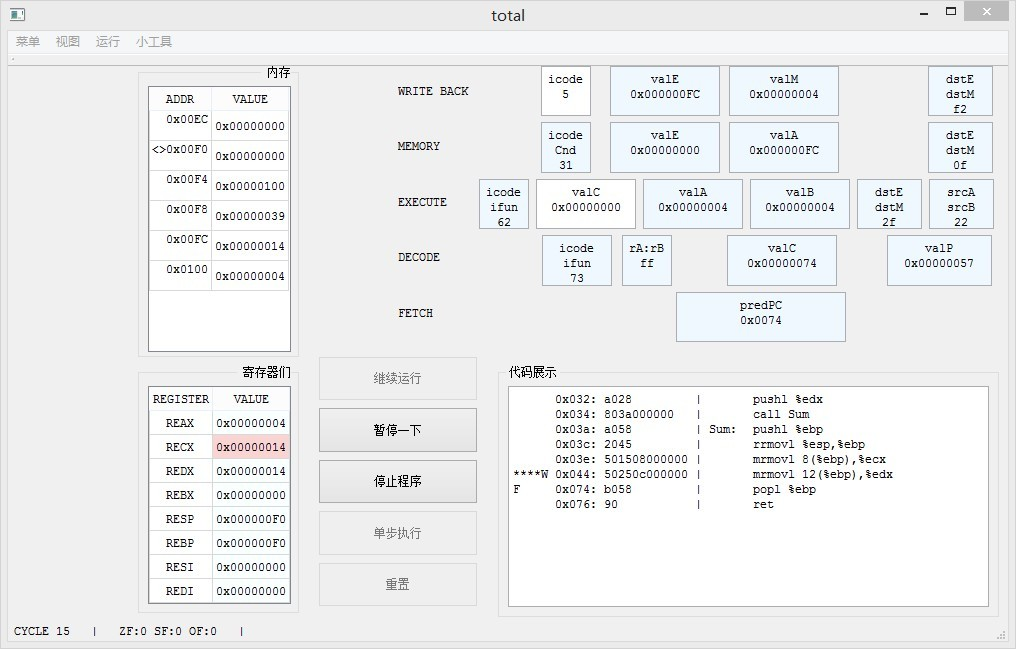
\includegraphics[width = 15cm]{2.jpg}
\end{center}

\begin{center}
程序运行时栈,用“<>”显示当前的栈帧(callee),同时还会显示caller的栈情况。

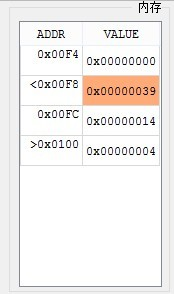
\includegraphics[width = 5cm]{3.jpg}
\end{center}

\begin{center}
8个寄存器对应的值。

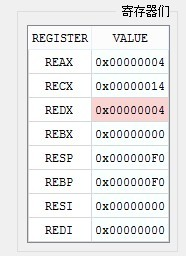
\includegraphics[width = 5cm]{4.jpg}
\end{center}
\begin{center}
流水线寄存器,这个周期没有用到的pipeline register会保持白色。
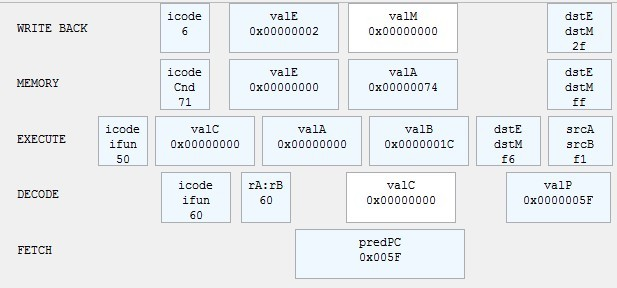
\includegraphics[width = 10cm]{5.jpg}
\end{center}

\begin{center}
代码展示,可以看到各个阶段当前执行到什么指令(下图初始全是在0x000处)
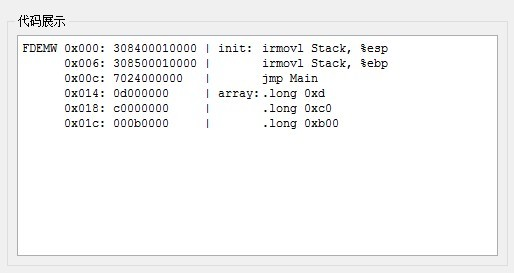
\includegraphics[width = 10cm]{6.jpg}
\end{center}

\begin{center}
下方有状态栏,显示出当前执行到第几个周期。如果遇到冒险会提示是怎样的hazard,同时会指示出程序的反应(bubble/stall)。
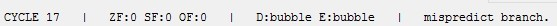
\includegraphics[width = 10cm]{7.jpg}
\end{center}

\subsection{怎样运行程序}
可以通过按屏幕中的按钮运行,也可以在菜单中调不同速率。

其中要说明的是停止的时候,虽然界面显示的值并不更新,但是下次继续运行的时候会从头开始。

另外并没有“后退一步”这种功能,因为普通的IDE都不会有这种功能。(一个CPU怎么能重置成历史时刻的数据?不符合实际,只能从头开始运行)
\subsection{菜单栏其他功能}
另外用户界面还有以下功能
\begin{enumerate}
\item 文件操作
\begin{itemize}
	\item 载入新的Y86指令文件
	\item 保存当前进度(内存和寄存器情况)到指定文件(我表示为.pk格式)
	\item 载入进度文件
	\item 导出结果到文件中,以txt的格式
\end{itemize}
\item 视图,提供几种不同的视图,能让用户看到他们只关心的内容
\begin{itemize}
	\item 全局视图
	\item 只看流水线寄存器
	\item 只看寄存器和内存
\end{itemize}
\item 运行
\begin{itemize}
	\item 以不同速率来运行,为了图形界面的显示效果(慢速运行的时候有颜色,如果颜色闪烁太快会对用户造成精神污染,所以我在快速运行的时候去掉颜色变化),这里只提供几种速度,单位是instruction per second(IPS)
	\item 运行,单步,暂停,停止等控制,同上。
\end{itemize}
\item 其他小工具,包括
\begin{itemize}
	\item 根据地址,读取当前内存对应的数据
	\item 直接修改内存的值
\end{itemize}
\end{enumerate}
\section{UI的关键实现}
\subsection{模拟运行}
为了后面程序更好的操作,我们把模拟器封装成一个类Simulator()。
Simulator包括以下方法
\begin{enumerate}
\item init() 初始化
\item step(update\_fun = None) 单步执行,同时把结果通过传入的update\_fun函数反馈到界面上
\item run\_all() 一次执行全部代码并输出
\end{enumerate}

在程序commit内存修改的时候,会调用update\_fun(addr, value),告诉UI界面需要更新addr这个内存/寄存器,刷新界面。

\subsection{颜色的更新}
在值改变的时候(可能)会有颜色变化,然后过了一段时间又会重新变成白色(类似于cool down),这样的功能使用CSS和HTML可以简单实现(比如说使用-webkit-transform等),然而我这次要用的是Qt,所以我手动实现了这个功能。
%continue here
\section{其他功能}
\section{遇到的问题}
\section{项目总结}
\section{Thank You}
\indent\indent
{\Large{
截至本报告完成的时候,代码已经没有任何bug。考虑到今天到明天还会继续整理和优化代码,可能在最终应用程序会引入一些小问题,请谅解。

View this project on GitHub\cite{2}

Report is written in \LaTeX}

\begin{thebibliography}{99}
\bibitem{1} \url{http://www.csapp.cs.cmu.edu/}
\bibitem{2} \url{https://github.com/kjkszpj/AE86}
\bibitem{3} \url{http://en.wikipedia.org/wiki/Endianness#Little-endian}
\end{thebibliography}

\end{document}